\documentclass[12pt, a4paper]{article}
\usepackage[utf8]{inputenc}
\usepackage{hyperref}
\usepackage{graphicx}
\usepackage{listings}
\usepackage{xcolor}
\usepackage{float}
\usepackage{caption}
\usepackage{subcaption}

\definecolor{codegreen}{rgb}{0,0.6,0}
\definecolor{codegray}{rgb}{0.5,0.5,0.5}
\definecolor{codepurple}{rgb}{0.58,0,0.82}
\definecolor{backcolour}{rgb}{0.95,0.95,0.92}

\lstdefinestyle{mystyle}{
    backgroundcolor=\color{backcolour},   
    commentstyle=\color{codegreen},
    keywordstyle=\color{magenta},
    numberstyle=\tiny\color{codegray},
    stringstyle=\color{codepurple},
    basicstyle=\ttfamily\footnotesize,
    breakatwhitespace=false,         
    breaklines=true,                 
    captionpos=b,                    
    keepspaces=true,                 
    numbers=left,                    
    numbersep=5pt,                  
    showspaces=false,                
    showstringspaces=false,
    showtabs=false,                  
    tabsize=2
}

\lstset{style=mystyle}

\hypersetup{
    colorlinks=true,
    linkcolor=black,
    urlcolor=cyan,
}

\graphicspath{{img/}}


\title{\textbf{Elaborato di Intelligenza Artificiale} \\ Implementazione di una Simulazione con Modelli di Reti Neurali Utilizzando l'Ambiente di Sviluppo Python}
\author{Soldà Matteo --- 1226319}
\date{\today}

\begin{document}

\begin{figure}
    \centering
    \includegraphics[width=0.50\textwidth]{Logo_Università_Padova}
\end{figure}

\maketitle

\newpage
\begin{abstract}
Nel presente elaborato verrà implementata una simulazione tramite modelli di reti neurali utilizzando l'ambiente di sviluppo Python.\\
La simulazione si baserà sul database \textit{MNIST}, riguardante il riconoscimento di numeri manoscritti, fornitoci durante la terza esercitazione pratica.\\
Dopo aver introdotto i vari tipi di rete e i loro risultati tramite un breve report, si cercherà rispondere a tre domande essenziali: definire le cifre più difficili da riconoscere, quantificare la variazione di accuratezza dovuta all'inserimento di rumore nel \textit{training pattern} e la variazione dell'accuratezza di riconoscimento sul \textit{testing pattern} riducendo drasticamente le dimensioni del \textit{training pattern}.    
\end{abstract}

\newpage
\tableofcontents

\newpage
\section{Introduzione}
In questo elaborato si prenderà in considerazione uno dei problemi più famosi che vengono sottoposti alle intelligenze artificiali: il riconoscimento di numeri manoscritti.
La simulazione chè verrà presentata si baserà sul dataset \textit{MNIST}, il quale contiene 70.000 immagini, con relative etichette, di cifre comprese tra 0 e 9 scritte a mano.\\
Per risolvere il problema sopra descritto, utilizzeremo due Percettroni Multi-Strato: la variante classica e quella convoluzionale.\\
Per testare entrambe le reti, suddivideremo il dataset in due parti: il training set composta da 60.000 immagini e il test set composto da 10.000 immagini. Dopo l'addestramento della rete, si procederà con la predizione, per poi passare ad una seconda predizione nel quale il test set conterrà del rumore crescente.

\newpage
\section{Costruzione della Rete Neurale e Test --- Breve Report}
\subsection{Multi Layer Perceptron --- Versione Classica}
Come prima rete, è stata creata un Percettrone Multi-Strato composto da 2 strati nascosti, ognuno dei quali formato da 500 neuroni. Effettuato l'addestramento su un massimo di 15 cicli e tramite funzione di attivazione "\textit{RELU}", la curva di apprendimento appare come sotto riportato:
\begin{figure}[H]
    \centering
    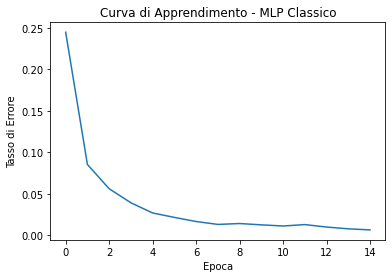
\includegraphics[width=0.50\textwidth]{Curva_MLP}
\end{figure}
Da notare che con soli 15 cicli di addestramento, si riceve un warning che ci avvisa del fatto che la rete non è riuscita a convergere. Probabilmente con un maggior numero di cicli, la rete potrebbe convergere.
Tramite la funzione \textit{score()}, si calcola che l'accuratezza della rete è fissata a \(97.79\%\).
Per completezza, è stato anche effettuato una predizione sullo stesso test set dove sono stati inseriti, in diversi step, 10 livelli di rumore compresi nell'intervallo \([0.1 , 1.0]\). Di seguito la variazione dell'errore all'aumentare del rumore:
\begin{figure}[H]
    \centering
    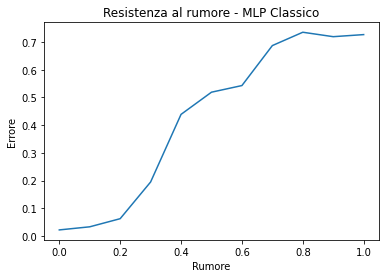
\includegraphics[width=0.50\textwidth]{Rumore_MLP.png}
\end{figure}

\subsection{Multi Layer Perceptron --- Versione Convoluzionale}
A seguire, è stata creata una variante convoluzionale di MLP formata da 2 strati convoluzionali così definiti:
\begin{itemize}
    \item Primo Strato: 18 filtri e un kernel \(3*3\)
    \item Secondo Strato: 28 filtri e un kernel \(4*4\)
\end{itemize}
Entrambi questi strati presentano una funzione di attivazione "\textit{RELU}".\\
Dopo aver addestrato la rete, la curva di apprendimento risulta essere:
\begin{figure}[H]
    \centering
    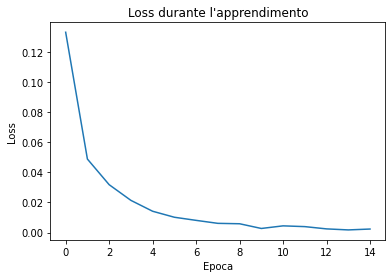
\includegraphics[width=0.50\textwidth]{Curva_Conv.png}
\end{figure}
Tramite la funzione di predizione abbiamo potuto constatare che l'accuratezza risulta essere del \(99.91\%\).\\
Anche in questo caso è stato effettuato il test su vari livelli di rumore e l'accuratezza al variare del rumore (in confronto con la versione classica) risulta essere:
\begin{figure}[H]
    \centering
    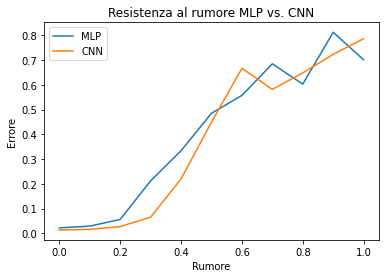
\includegraphics[width=0.50\textwidth]{Rumore_Conv.png}
\end{figure}

Essendo normalmente le MLP Convoluzionali maggiormente adatta per la classificazione di immagini, si è provato ad aggiungere del rumore anche durante l'addestramento della rete.\\
L'addestramento verrà effettuato su un livello di rumore pari a \(0.5\) e poi verrà testata l'affidabilità sul test set con 10 livelli di rumore.\\
Dal test, emerge quanto successivamente mostrato:
\begin{figure}[H]
    \centering
    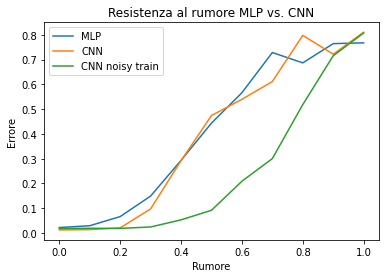
\includegraphics[width=0.50\textwidth]{Rumore_Conv_Add.png}
\end{figure}

\subsection{Risultati}
Dai precedenti test, si può concludere che, su questo tipo di dataset e con i parametri preimpostati, su di un addestramento di 15 cicli, le due varianti di MLP si assomigliano, non mostrando grandi differenze nell'accuratezza sul test set. I risultati migliori si ottengono addestrando la variante convoluzionale con del rumore.

\newpage
\section{Primo Quesito --- Numeri Difficili da Riconoscere}
\subsection{Visualizzazione di Pattern Erronei}
Per poter visualizzare al meglio le previsioni sbagliate, utilizzeremo tre liste di supporto:
\begin{itemize}
    \item sbagliate[]: contiene le "immagini" originali
    \item previsto[]: contiene il valore previsto dalla rete
    \item target[]: contiene il valore target associato al valore originario
\end{itemize}

Inizialmente verrà utilizzata una MLP classica, a seguire saranno mostrati anche i risultati della variante convoluzionale.
Di seguito i risultati:
\begin{figure}[H]
    \centering
    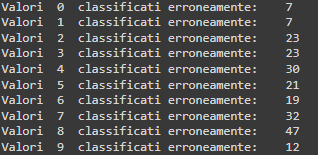
\includegraphics[width=0.50\textwidth]{ErrateClassica.png}
\end{figure}

Nella simulazione risulta che il numero che viene classificato più volte erroneamente è \(8\), che conta un numero di classificazioni errate di \(47\). A seguire il numero \(7\) e poi il \(4\). I numeri che invece vengono classificati in modo sbagliato poche volte sono \(0\), \(1\) e \(9\).\\
Di seguito alcuni esempi di numeri \(8\) che sono stati classificati in modo erroneo:

\begin{figure}[H]
    \centering
    \begin{subfigure}{.5\textwidth}
        \centering
        \caption{Numero Previsto: 0}
        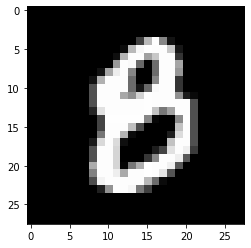
\includegraphics[width=0.50\textwidth]{otto1.png}
    \end{subfigure}% 
    \begin{subfigure}{.5\textwidth}
        \centering
        \caption{Numero Previsto: 4}
        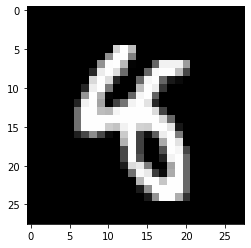
\includegraphics[width=0.50\textwidth]{otto2.png}
    \end{subfigure} 
\end{figure}

\begin{figure}[H]
    \begin{subfigure}{.5\textwidth}
        \centering
        \caption{Numero Previsto: 7}
        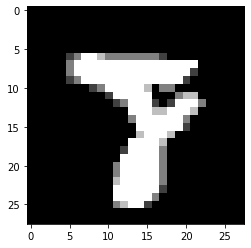
\includegraphics[width=0.50\textwidth]{otto3.png}
    \end{subfigure} %
    \begin{subfigure}{.5\textwidth}
        \centering
        \caption{Numero Previsto: 4}
        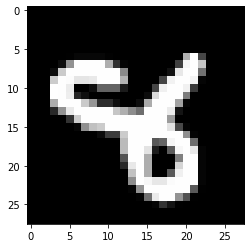
\includegraphics[width=0.50\textwidth]{otto4.png}
    \end{subfigure} 
\end{figure}

\begin{figure}[H]
    \centering
    \caption{Numero Previsto: 9}
    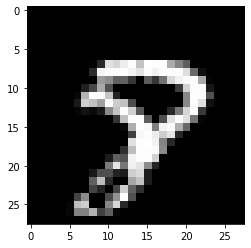
\includegraphics[width=0.25\textwidth]{otto5.png}
\end{figure} 

Per quanto riguarda la variante convoluzionale, si è utilizzato lo stesso metodo sopra descritto per l'estrazione dei valori classificati erroneamente e i risultati sono stati i seguenti:
\begin{figure}[H]
    \centering
    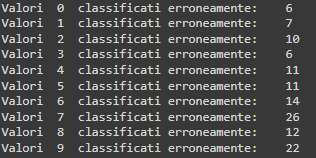
\includegraphics[width=0.50\textwidth]{ErrateConv.png}
\end{figure}
A differenza di quanto visto prima, i numeri che vengono mal classificati per la maggiore sono i \(9\) che contano un numero di classificazioni errate pari a 22. Da notare come il numero di classificazioni errate sia molto minore rispetto alla variante classica.\\
Di seguito alcuni esempi di \(9\) classificati erroneamente:

\begin{figure}[H]
    \begin{subfigure}{0.5\textwidth}
        \centering
        \caption{Numero Previsto: 5}
        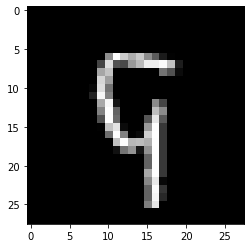
\includegraphics[width=0.50\textwidth]{nove1.png}
    \end{subfigure}
    \begin{subfigure}{0.5\textwidth}
        \centering
        \caption{Numero Previsto: 7}
        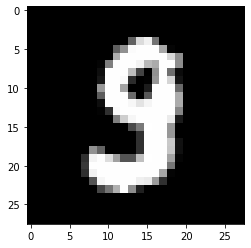
\includegraphics[width=0.50\textwidth]{nove2.png}
    \end{subfigure}
\end{figure}

\begin{figure}[H]
    \begin{subfigure}{0.5\textwidth}
        \centering
        \caption{Numero Previsto: 3}
        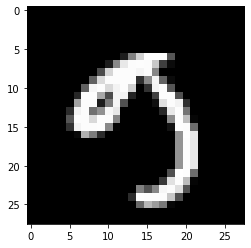
\includegraphics[width=0.50\textwidth]{nove3.png}
    \end{subfigure}
    \begin{subfigure}{0.5\textwidth}
        \centering
        \caption{Numero Previsto: 1}
        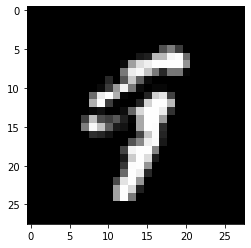
\includegraphics[width=0.50\textwidth]{nove4.png}
    \end{subfigure}
\end{figure}
\begin{figure}[H]
    \centering
    \caption{Numero Previsto: 1}
    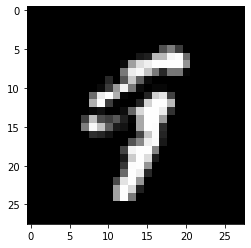
\includegraphics[width=0.25\textwidth]{nove5.png}
\end{figure}

\subsection{Aggiunta di Rumore in Pattern Corretti}
Per procedere con il quesito, prima di aggiungere del rumore, creiamo due nuove liste che conterranno le immagini e i target delle immagini che la rete ha classificato correttamente.\\
Il test è stato eseguito rumore crescente. La rete sarà considerata "affidabile" sino a quando il rateo di \textit{true positive} sarà maggiore del \(75\%\).\\
Per quanto riguarda la variante classica, la variazione dell'accuratezza risulta essere:
\begin{figure}[H]
    \centering
    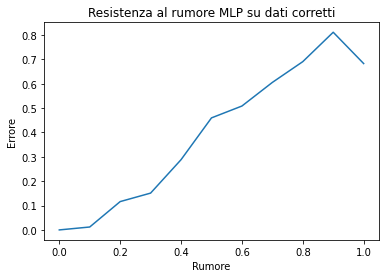
\includegraphics[width=0.50\textwidth]{TPClassica.png}    
\end{figure}
In linea con quanto precedentemente detto, la rete sarà considerabile come affidabile finché il rumore sarà compreso tra i valori \([0.0, 0.3]\), estremi compresi.\\
Di seguito alcuni esempi di valori classificati in modo errato:

\begin{figure}[H]
    \begin{subfigure}{0.5\textwidth}
        \centering
        \caption{Target: 7 - Previsto: 3}
        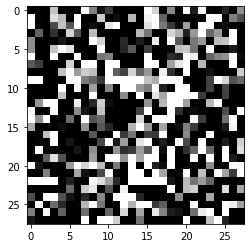
\includegraphics[width=0.5\textwidth]{ErrClass1.png}
    \end{subfigure}
    \begin{subfigure}{0.5\textwidth}
        \centering
        \caption{Target: 0 - Previsto: 5}
        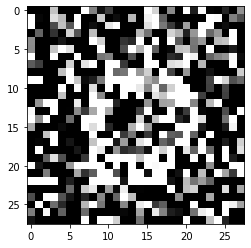
\includegraphics[width=0.5\textwidth]{ErrClass2.png}
    \end{subfigure}
\end{figure}

\begin{figure}[H]
    \begin{subfigure}{0.5\textwidth}
        \centering
        \caption{Target: 6 - Previsto: 5}
        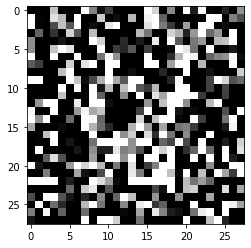
\includegraphics[width=0.5\textwidth]{ErrClass3.png}
    \end{subfigure}
    \begin{subfigure}{0.5\textwidth}
        \centering
        \caption{Target: 1 - Previsto: 2}
        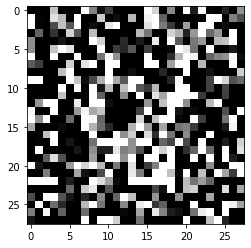
\includegraphics[width=0.5\textwidth]{ErrClass4.png}
    \end{subfigure}
\end{figure}

\begin{figure}[H]
    \centering
    \caption{Target: 1 - Previsto: 5}
    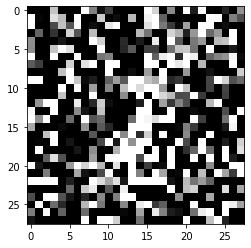
\includegraphics[width=0.25\textwidth]{ErrClass5.png}
\end{figure}

Per quanto riguarda la variante convoluzionale, il risultato risulta essere:
\begin{figure}[H]
    \centering
    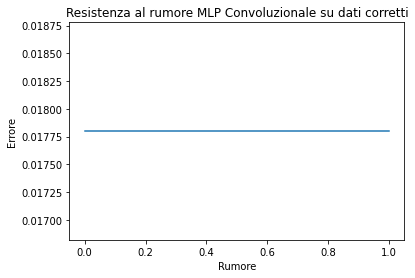
\includegraphics[width=0.50\textwidth]{TPConv.png}
\end{figure}

Sorprendetemente, il livello di accuratezza rimane stabile intorno al \(0.9822\), per cui la rete rimarrà affidabile per tutti i valori di rumore compresi tra \([0.0, 1.0]\).\\
Di seguito alcuni esempi di valori classificati erroneamente:
\begin{figure}[H]
    \begin{subfigure}{0.5\textwidth}
        \centering
        \caption{Target: 3 - Previsto: 9}
        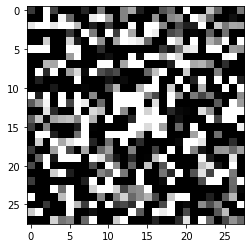
\includegraphics[width=0.5\textwidth]{ErrConv1.png}
    \end{subfigure}
    \begin{subfigure}{0.5\textwidth}
        \centering
        \caption{Target: 0 - Previsto: 3}
        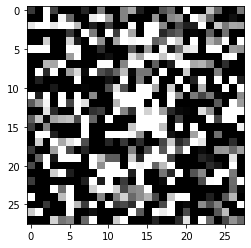
\includegraphics[width=0.5\textwidth]{ErrConv2.png}
    \end{subfigure}
\end{figure}

\begin{figure}[H]
    \begin{subfigure}{0.5\textwidth}
        \centering
        \caption{Target: 1 - Previsto: 2}
        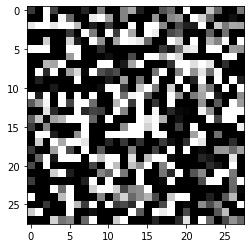
\includegraphics[width=0.5\textwidth]{ErrConv3.png}
    \end{subfigure}
    \begin{subfigure}{0.5\textwidth}
        \centering
        \caption{Target: 0 - Previsto: 2}
        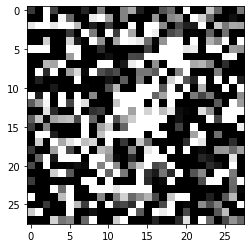
\includegraphics[width=0.5\textwidth]{ErrConv4.png}
    \end{subfigure}
\end{figure}

\begin{figure}[H]
    \centering
    \caption{Target: 8 - Previsto: 9}
    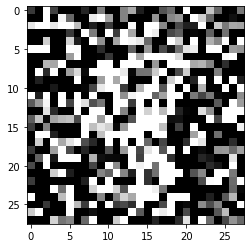
\includegraphics[width=0.25\textwidth]{ErrConv5.png}
\end{figure}

\newpage
\section{Secondo Quesito --- Variazione dell'Accuratezza su Addestramento Rumoroso}
\paragraph{Warning:} Dato che nella sezione saranno definite molte MLP, onde evitare tempi di attesa troppo lunghi, le iterazioni massime sono state ridotte da 15 a 5. La necessità di creare nuove MLP è data dal fatto che il sovrapporsi di addestramenti sulla stessa rete potrebbe influire positivamente sulla predizione e creare di conseguenza dei falsi positivi dato che non si saprà quale degli addestramenti ha massimizzato la resa.
\subsection{Accuratezza su di un Pattern di Test dopo Addestramento Rumoroso}
Prima di tutto, verranno inizializzate 10 MLP, ognuna delle quali sarà addestrata per un singolo e diverso rumore. Di seguito le curve di apprendimento delle reti:
\begin{figure}[H]
    \begin{subfigure}{0.5\textwidth}
        \centering
        \caption{Rumore 0.1}
        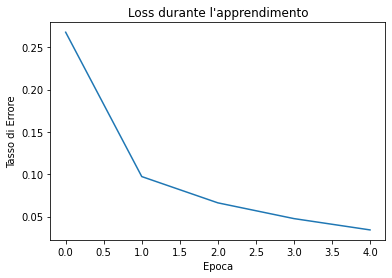
\includegraphics[width=0.80\textwidth]{Rumore1.png}
    \end{subfigure}
    \begin{subfigure}{0.5\textwidth}
        \centering
        \caption{Rumore 0.2}
        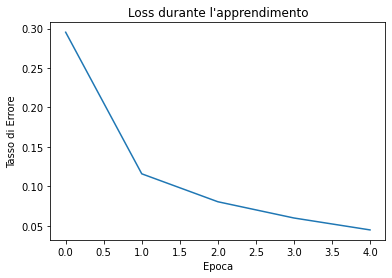
\includegraphics[width=0.80\textwidth]{Rumore2.png}
    \end{subfigure}    
\end{figure}

\begin{figure}[H]
    \begin{subfigure}{0.5\textwidth}
        \centering
        \caption{Rumore 0.3}
        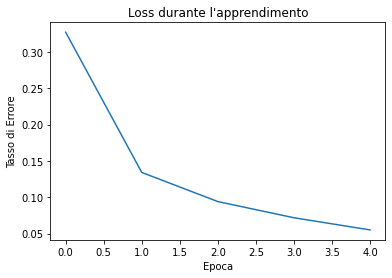
\includegraphics[width=0.80\textwidth]{Rumore3.png}
    \end{subfigure}    
    \begin{subfigure}{0.5\textwidth}
        \centering
        \caption{Rumore 0.4}
        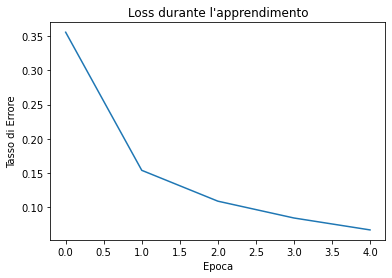
\includegraphics[width=0.80\textwidth]{Rumore4.png}
    \end{subfigure}  
\end{figure}  

\begin{figure}[H]
    \begin{subfigure}{0.5\textwidth}
        \centering
        \caption{Rumore 0.5}
        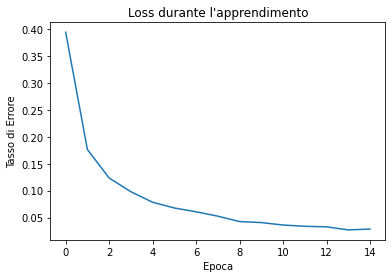
\includegraphics[width=0.80\textwidth]{Rumore5.png}
    \end{subfigure}    
    \begin{subfigure}{0.5\textwidth}
        \centering
        \caption{Rumore 0.6}
        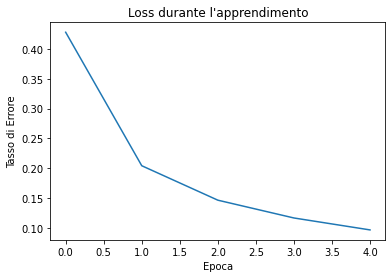
\includegraphics[width=0.80\textwidth]{Rumore6.png}
    \end{subfigure}  
\end{figure}

\begin{figure}[H]
    \begin{subfigure}{0.5\textwidth}
        \centering
        \caption{Rumore 0.7}
        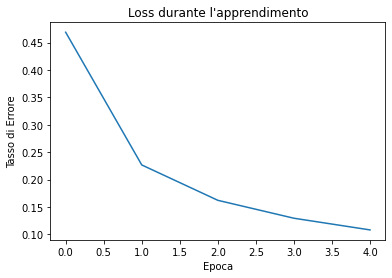
\includegraphics[width=0.80\textwidth]{Rumore7.png}
    \end{subfigure}    
    \begin{subfigure}{0.5\textwidth}
        \centering
        \caption{Rumore 0.8}
        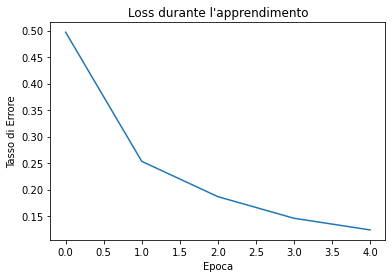
\includegraphics[width=0.80\textwidth]{Rumore8.png}
    \end{subfigure}  
\end{figure}

\begin{figure}[H]
    \begin{subfigure}{0.5\textwidth}
        \centering
        \caption{Rumore 0.9}
        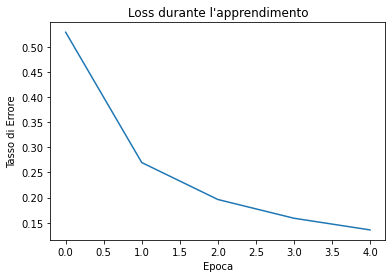
\includegraphics[width=0.80\textwidth]{Rumore9.png}
    \end{subfigure}    
    \begin{subfigure}{0.5\textwidth}
        \centering
        \caption{Rumore 0.10}
        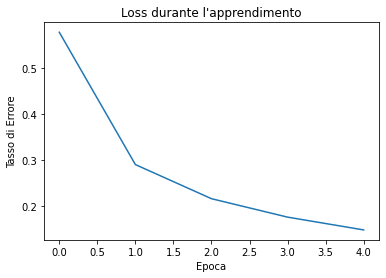
\includegraphics[width=0.80\textwidth]{Rumore10.png}
    \end{subfigure}       
\end{figure} 

\subsection{Definizione di un Valore di Rumorosità Ottimale}
Allo stato attuale, l'accuratezza della MPL classica al variare del rumore risulta:
\begin{itemize}
    \item Rumore 0.1: 0.6258
    \item Rumore 0.2: 0.5855
    \item Rumore 0.3: 0.5847
    \item Rumore 0.4: 0.5826
    \item Rumore 0.5: 0.6005
    \item Rumore 0.6: 0.4644
    \item Rumore 0.7: 0.4529
    \item Rumore 0.8: 0.4305
    \item Rumore 0.9: 0.4958
    \item Rumore 1.0: 0.4208
\end{itemize}

Di conseguenza, i due rumori che massimizzano la resa della rete sono \(0.1\) e \(0.5\).

\newpage
\section{Terzo Quesito --- Variazione dell'Accuratezza su Pattern di Addestramento Ridotto}
\subsection{50\% del Training Set}
\subsection{25\% del Training Set}
\subsection{10\% del Training Set}


\end{document}
